% !TEX root = ../master.tex
\chapter{Implementation}
\label{chap:impl}

The previous chapter yielded a general execution plan that shall implemented in the coming 
section while utilizing the cluster computer at the \ac{DHBW}. 
For each implementation detail the specifically chosen values are given during the process. Each of the steps holds 
the possibilities for errors which will also be evaluated.
The outcome of the taken steps is only a partially functional Hadoop cluster.
The reasons and implications for this restricted outcome are given.
Suggestions for future projects how better results might be achieved is given in the end.

\section{Infrastructure Set-Up in OpenStack}

The foundation for the cluster architecture that has been illustrated in figure \vref{fig:architecture} are the host \acp{VM}, their storage and the network that connects them.
In the course of this process some minor adaptions are made to the proposed architecture.
Especially the \texttt{hadoop-master-0} node now also runs the \ac{HDFS} Datanode and YARN Nodemanager service and therefore has a storage volume attached to it.

To set up the cluster the web interface of OpenStack can be used, which is accessible at
\urlinline{https://controller.c4.dhbw-mannheim.de/} from within the \ac{DHBW} network.
Each operation on the infrastructure can be performed within this interface.

\subsection{Execution}

\subsubsection{Firewall Rules}

The firewall in OpenStack can be configured by creating \emph{security groups}.
These security groups describe rules for allowing and prohibit outgoing and incoming connections.
For this project two security groups are created and assigned to each of the \acp{VM}.
THe first group deals with \emph{default} settings. It allows all outgoing connections 
and allows incoming connections on port 22, which is the port used for \ac{SSH} access, 
as well as incoming ping packages in the Internet Control Message Protocol.
The second group deals with Hadoop specific ports.
A detailed over all necessary ports is given by \textcite{hortonworks2017reference} in their port reference.
However to make development and access more flexible, this group does temporarily 
allow all incoming requests.

\subsubsection{Network}

To enable an interconnection between the nodes in the cluster it is useful to create a private network between them.
The network uses the address space of 10.100.10.0/24 which is a subnet of the private address space defined in RFC~1918 by the the Internet Engineering Task Force \autocite[][]{ietf1996rfc1918}.
Figure \ref{fig:networks_subnets} lists all the networks that are available after the internal network is created. 
The network named \emph{int-net-10} is the internal network which all nodes connect to. Furthermore all nodes need to connect to the \emph{ext-net-201} network which allows them to connect to the Internet and makes them accessible from within the \ac{DHBW} network.

\begin{table}[hbt]
\resizebox{\textwidth}{!}{%
	\begin{tabular}{lll}
	  Network Name & Sub-networks & Description\\
	  \hline
	  ext-net-201 & 141.72.191.0/24 & Pre-configured connection to \ac{DHBW} internal network\\
	  ext-net-112 & 192.168.112.0/20 & Pre-configured connection with unknown connectivity\\
	  int-net-10 & 10.100.10.0/24 &  New internal network used by Hadoop\\
	\end{tabular}%
	}
	\caption{Sub-networks within the project in OpenStack}
	\label{fig:networks_subnets}
\end{table}

\begin{figure}[hbt]
  {\centering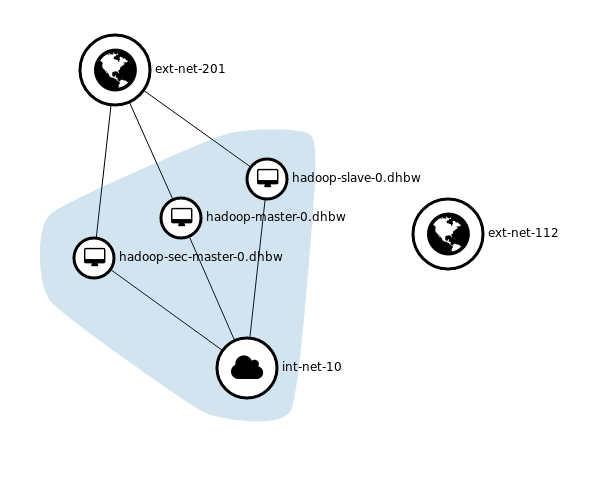
\includegraphics[width=0.8\textwidth]{{img/network_topology}.png}\par}
  \caption{Network topology created in OpenStack}
  \label{fig:network_topology}
\end{figure}

Once the nodes are created, the network topology looks like figure \ref{fig:network_topology}. The highlighted denotes the network connections that exists purely in OpenStack and have no physical connection to any outside network.
The figure also shows the names of the hosts and the network names.

\subsubsection{Virtual Machines}

In the next step the virtual machines are created.
The OpenStack environment offers different \emph{flavors} of instance sized for the \acp{VM} which is a pre-configured combination of resources associated to it.
To create a node the developer can chose from the presets listed in table \ref{fig:instance_sizes}. The flavors differ in amount of \acp{VCPU}, \ac{RAM} and root storage.
The set-up of the hosts is done for each node individually, 
since the names and flavor configurations differ between them.
The names are respective to proposed architecture but have a \emph{dhbw} domain ending 
added to them, which is not officially registered but is necessary for Ambari to identify the hosts correctly.


\begin{table}[hbt]
\centering
\resizebox{0.8\textwidth}{!}{%
	\begin{tabular}{lrrr}
	  Instance Flavor Name & \acp{VCPU} & \acs{RAM} & Root Disk Size \\
	  \hline
	  m1.nano & 1 & 64~\acs{MB} & 1~\acs{GB} \\
	  m1.tiny & 1 & 512~\acs{MB} & 5~\acs{GB} \\
	  m1.small & 1 & 1~\acs{GB} & 10~\acs{GB} \\
	  m1.medium & 2 & 2~\acs{GB} & 20~\acs{GB} \\
	  m1.large & 4 & 4~\acs{GB} & 40~\acs{GB} \\
	  m1.xlarge & 8 & 8~\acs{GB} & 80~\acs{GB} \\
	\end{tabular}%
	}
	\caption{Available instance sizes in the \ac{DHBW} OpenStack environment}
	\label{fig:instance_sizes}
\end{table}


\begin{table}[hbt]
\centering
	\begin{tabular}{lrl}
	  Resource Type & Amount & Unit\\
	  \hline
	  Instances & 10 & \\
	  \acp{VCPU} & 20 & \\
	  \acs{RAM} & 51200 & \acs{MB} \\
	  Floating \acs{IP} Addresses & 10 & \\
	  Security Groups & 10 & \\
	  Volumes & 10 & \\
	  Volume Storage & 1000 & \acs{GB}
	\end{tabular}
	\caption{Available resources for the project in the \ac{DHBW} OpenStack environment}
	\label{fig:resources_openstack}
\end{table}

Table \ref{fig:resources_openstack} describes how many resources are available at maximum for the project in the \ac{DHBW} OpenStack environment. The chosen configurations may in sum not exceed this limit.
As visible in table \ref{fig:instance_sizes} all instance of m1.small and larger have a core to memory ration of \emph{1~core~:~1~GB~RAM}, which means that, if all 20 available cores are used, only 20 out of 51,2 GB RAM  can be used. It is favourable to have maximum sized \acp{VM} with respect to memory to give Hadoop the possibility make better use of it.
Therefore the best allocation for the nodes is to use a m1.xlarge instance for the master node, a m1.xlarge for the secondary and a large instance for the slave node.
This in sum gives 20 \acp{VCPU} and 20~\ac{GB} \ac{RAM} and no further cores are available to allocate more nodes.


Each instance is using the Ubuntu 16.04 operating system which is compatible with \ac{HDP}, Ambari and Hadoop. As discussed before the security groups for default access and hadoop specific access are assigned to the hosts, and they are connected to the internal and external network. An \ac{SSH} key is used for authentication.
The successful creation of each host is tested by accessing it via \ac{SSH} using the specified key and the user \emph{ubuntu}.


\subsubsection{Storage}

In order for the Hadoop cluster to store \ac{HDFS} data it is necessary to split up the available 1000~\ac{GB} for storage into three volumes, one for each host.


TODO
create disks
assing them
format them
ansible will be used to mount them

\subsection{Encountered Issues and Lessons Learned}

Access to the 

TODO Access only from dhbw on site net leads to difficult development conditions where author needs to be on site and is restricted by the locality

TODO Network connection unstable leading to more difficult environment with regular loss of connectivity to server

TODO Internal errors within openstack (temporary) where not enough resources could be allocated to get the requested VMs, later resolved

TODO when encountering resource issues, tried on BW cloud again to train


\section{System Set-Up with Ansible}

TODO ansible script already used in chapter 3 so now it is adapted to the new needs

\subsection{Preparation}

TODO
TODO explain and maybe print this particular playbook yes yes print it with explainations
TODO maybe appendix
TODO Ansible
see \urlinline{https://github.com/XOSplicer/studienarbeit-hadoop-cluster-ansible}
     (in implementation explain how the ansible part works). 
     


\subsection{Execution}

TODO prepare hosts by running setup script
TODO apply ansible playbook
reboot for safty

\subsection{Encountered Issues and Lessons Learned}

TODO
literary none?

\section{Hadoop Set-Up with Ambari}

TODO

TODO Tools will be Apache Spark, Storm, Hive und Pig

\subsection{Preparation}
TODO

\subsection{Execution}
TODO

TODO ,  when promted to select nodes use manual registaration: reason dont upload ssh private key for root access 

\subsection{Encountered Issues and Lessons Learned}
TODO

TODO as expected the larger root partition of 80 GB was enough for the selected services

TODO memory on master node was exceeded even with not all services runnig (only)

TODO network DNS issues lead to failing installation, ha been re-done

TODO services crash due to memory shortage, generel unstable


\section{System Tests}

TODO

\subsubsection{Terasort}

TODO and \autocite{omally2008terasort}
TODO \urlinline{https://hadoop.apache.org/docs/r1.0.4/api/org/apache/hadoop/examples/terasort/TeraGen.html}\\urlinline{https://www.systutorials.com/3235/hadoop-terasort-benchmark/} (also mentioned in \autocite[][]{white2015hadoop})

\subsubsection{Ambari Service Checks}

TODO

HDFS WORKS
YARN is broken (sometimes)
mapred is broken (sometimes)

check successfull where service is up, not all services up. TODO which ones

\section{Conclusion}



During the implementation of the prject the \ac{DHBW} Cloud environment showed unreliablities that influenced
TODO dhbw cloud is unreliable af

TODO process is way too hard for and too long for students to do in a lecture without depper understanding of sysadmin  

TODO NOT scuccessfull because of ??????????

TODO Abweichen von architecture war dumm, da memory knapp durch zu viele prozesse

TODO maintainability is fucked, just let professsionals do it










